\documentclass[journal]{IEEEtran}

% *** CITATION PACKAGES ***
\usepackage[style=ieee]{biblatex} 
% \bibliography{example_bib.bib}    %your file created using JabRef

% *** MATH PACKAGES ***
\usepackage{amsmath}

% *** PDF, URL AND HYPERLINK PACKAGES ***
\usepackage{url}
% correct bad hyphenation here
\hyphenation{op-tical net-works semi-conduc-tor}
\usepackage{graphicx}  %needed to include png, eps figures
\usepackage{float}  % used to fix location of images i.e.\begin{figure}[H]

\begin{document}

% paper title
\title{Non-Invasive Smart Energy Monitoring System}

% author names 

\author{Shridatha Hegde, 
        Akhilesh Kumbhar,
        Sagar Patil,
        Sai Preetham M,
        Saiprasanna Kuragodi 
        {\newline \begin{center}
            \textbf{School of Electronics and Communication, KLE Technological University- Hubballi}
        \end{center}}}% <-this % stops a space

% The report headers
\markboth{VI Semester Minor Project, 2020-2021}%do not delete next lines
{Shell \MakeLowercase{\textit{et al.}}: Bare Demo of IEEEtran.cls for IEEE Journals}

% make the title area
\maketitle

% As a general rule, do not put math, special symbols or citations
% in the abstract or keywords.
\begin{abstract}
Internet exploration has changed the world completely. This has brought people closer than ever before. The breakthrough in computing and networking technologies takes the Internet of Things (IoT) to the next generation. Due to the growing number of communities and rapid
urbanization, the towns must revolutionize and remodel to smart cities that can be achieved with the help of the Internet of Things. Electricity usage has always been a concern for homes, institutions, and business owners. As resources become more scarce and electricity costs continue to rise, institutions and businesses need to be aware of how they are utilizing their energy and how they can use it more efficiently. Non -invasive based current measuring sensors are used to measure the energy consumed by a particular appliance/equipment. The sequence-based algorithms with LSTM neural networks are used to diagnose and forecast energy consumption in traditional commercial and residential energy systems. The system is integrated with cloud computing technologies to identify times of high usage and real-time monitoring.
\end{abstract}

\begin{IEEEkeywords}
non-invasive, energy, cloud, LSTM, IoT.
\end{IEEEkeywords}

\section{Introduction}
\IEEEPARstart The electricity bill generated by the electricity supply company can be often confusing as it does not explain the consumption of individual rooms or labs or cabins but instead, the bill provides a sum of all these as a whole. So this paper as a whole tries to explain the power consumed individually by these sections. Predicting the possible power consumption is a very important job at hand as this helps to plan the consumption accordingly. Using different machine learning algorithms, these possible future values would be sought. Main objectives being to design and develop a data acquisition system for energy consumption measurement, to visualize and forecast consumption usage with cloud computing and to make energy monitoring smarter.

\section{Methodology}
  The proposed energy monitoring framework is based on Context-awareness. In this paper, Context-awareness is accomplished considering the profiles and inferring rules for each section of an institution.
  \newline
 
\textbf{A. Framework}
\newline
The framework consists of two layers and performs various functions including those of Figure 1. First, the data collection and control layer consists of non-invasive current sensors and an ESP32 controller. The Sensors collect the current usage (in Amp) and the controller performs energy consumption data calculation (in KWh). The data is stored in a cloud service database. 
 
\begin{figure}[H]%[!ht]
\begin {center}
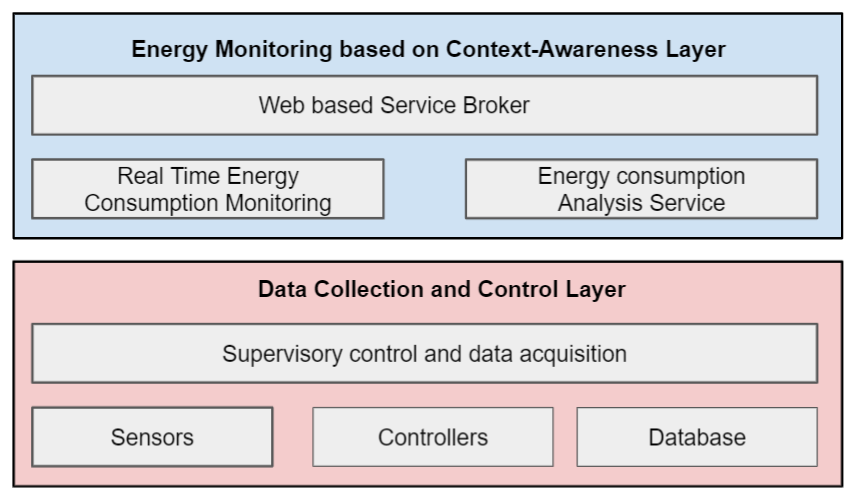
\includegraphics[width=9cm,height=5cm]{images/ieee fig1.png}
\caption{The proposed energy monitoring framework}
\end {center}
\end{figure}
The database has the tables for the raw data and converted data from the sensors. The energy management based on context-awareness layer administrates databases (DBs), with a front-end web interface for real-time data visualization for the user. Also with the employment of deep learning neural network-based model, analyses the past and present energy consumption and predicts future energy consumption. Also, the layer generates the
improved methods of energy management and forecasts the effects and performance indicators.
\newline

\textbf{B. Configuration}
\newline
The Configuration for the energy monitoring is shown in Figure 2. The Institution includes many kinds of new items to detect the energy consumption context, provides data to the institutional energy monitoring system (IEMS). IEMS collects data, analyses them, infers the context, and manages DBs. Users can be provided energy management services including monitoring, alarm, and forecast.

 \begin{figure}[H]%[!ht]
\begin {center}
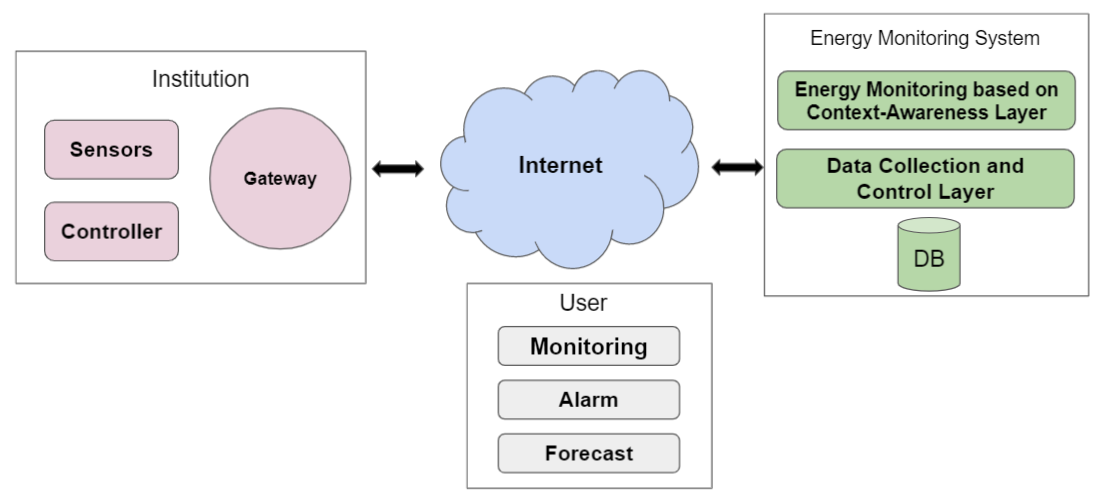
\includegraphics[width=9cm,height=4.5cm]{images/iee fig2.png}
\caption{Configuration and message flow framework}
\end {center}
\end{figure}

\section{Results and Discussion}
Literature survey of different papers and publications yielded the decision matrix for selecting the best-suited system for proof of concept. \par
SCT 012-30A is a non-invasive current transformer sensor used to calculate the amount of current flowing through a wire using the concept of the hall effect. This is a 30A 1V output sensor. Two resistors of the same within the range of 100 ohms to 470k ohm value to generate a voltage divider circuit which helps in the calibration of values. Efficient use of power is a concern that should not be neglected. ESP32 uses 240mA in active mode, this small number can be problematic in the long run, thus to control the power consumption configurable sleep power modes were implemented as optimized power management of the system.\par
Various prediction models including both statistical and machine learning were taken into consideration for appropriate trade-off. The usage of the deep learning approach resulted in better forecast accuracy of the model.
\newline 
  \begin{table}[!ht] %[H]
  \centering
  \label{table:Exps}
  \begin{tabular}{ll}
   Model &  Accuracy \\ \hline
   ARMA &    57\% \\
   Prophet &   59.42\% \\
   LSTM &   95\% \\
 \end{tabular}
 \caption{Performance of different models}
 \end{table}
\newline
Time-series forecasting is one of the major building blocks of Machine Learning. It is a sequence of data points taken at successive, equally-spaced points in time that can be used to predict the future. A time-series analysis model using LSTM deep learning architecture involves using historical data to forecast the future based on long short term memory with RNN as the base. It looks dataset for features such as trends, cyclical fluctuations, seasonality, and behavioural patterns.





\section{Summary}
In this paper, we added new contributions besides summarizing the IoT framework for smart energy in buildings. The work includes (1) energy consumption data analysis (2) experimental prototype that applies IoT networking and cloud computing technologies to help in judicial use of the energy. We put them into complete two-step research and added significant new contributions proving the ideas and concepts we proposed. By building this IoT framework in institutions, we aim to enable not only multi-scale energy proportionality, but also create an intelligent space that is an important part of the future smart world. We envision that the idea will provide not only significant economic benefits but also huge social benefits in terms of global sustainability. Using the framework, energy leakage can be reduced and the energy consumption is efficiently managed.

% \section*{Appendix}
% The system framework including both hardware and software service sections are pictorially depicted in this section.

%  \begin{figure}
% \begin {center}
% 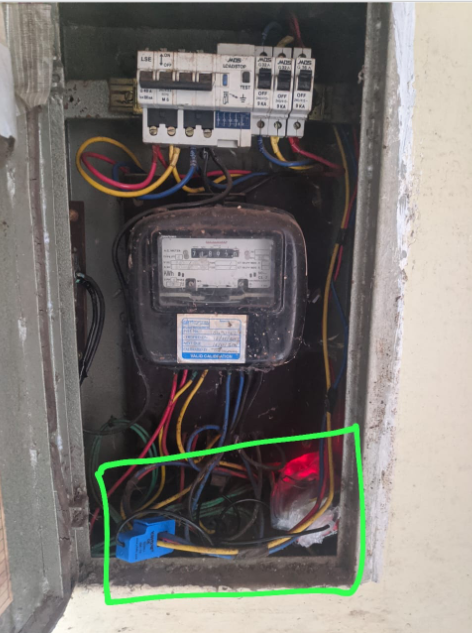
\includegraphics[width=5cm,height=8cm]{images/setup.png}
% \caption{Sensor Node}
% \end {center}
% \end{figure}

%  \begin{figure}
% \begin {center}
%   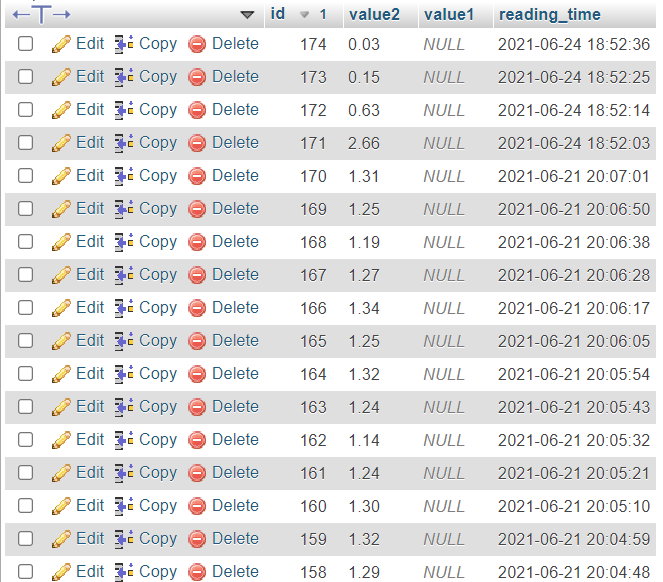
\includegraphics[width=6cm,height=5cm]{images/table.png}  
%   \caption{Database}
%   \end {center}
% \end{figure}

\newpage
\section*{Acknowledgment}
We express our deep sense of gratitude to \textbf{Dr. Ashok Shettar}, Vice-Chancellor, \textit{KLE Technological University}, and \textbf{Dr.Nalini C. Iyer}, Head of the department, \textit{School of Electronics and Communication Engineering} for providing the necessary facilities required for completion of this project and their exemplary guidance, monitoring and constant encouragement throughout the course of this project. We would also like to express our sincere gratitude towards our project guides \textbf{Dr. Sunita V. B} and \textbf{Dr. Saroja V. S} whose constant guidance and care made the project successful.


\section*{References}
[1] Adela Has, Marijana Zeki Susac Machine learning based system for managing energy efficiency of public sector as an approach towards smart cities.
 \newline
[2] A Santollamazza, V Introna Anamoly Detection in Energy Consumption for Compressed Air Generation systems: an approach based on artificial neural networks.
 \newline
[3] Jianli Pan, Raj Jain, Subharthi Paul, Tam Vu, Abusayeed Saifullah An Internet of Things Framework for Smart Energy in Buildings: Designs, Prototype, and Experiments.
 \newline
[4] Qing Yang, Hao Wang Privacy-Preserving Transactive Energy Management for IoT-aided Smart Homes via Blockchain.
 \newline
[5] Hyunjeong Lee, Sangkeun Yoo, Yong-Woon Kim An Energy Management Framework for Smart Factory based on Context-awareness.
 \newline
[6] Amam Hossain Bagdadee A Brief Review of the IoT-Based Energy Management System in the Smart Industry.
 \newline
[7] Dr. Rudra Kalyan Nayak, Dr. Ramamani Tripathy An Overview of Deep Learning in Smart Grids.
 \newline
[8] Syed Saqib Ali and Bong Jun Choi State-of-the-Art Artificial Intelligence Techniques for Distributed Smart Grids.
 \newline
[9] Naser Hossein Motlagh, Mahsa Mohammadrezaei and Julian Hunt Internet of Things (IoT) and the Energy Sector.
 \newline
[10] Mark Ditsworth, Manish Niraula Machine Learning based Energy Management System for grid disaster mitigation


\end{document}


